\kommentar{(Ent-)Laden Kondensator} %Thema
  
\begin{karte}{Wie heisst die Gleichung der folgender Entladefunktion?\\ %Autor: Simon Walker
%Version: 1.0
%Datum: 10.11.2019

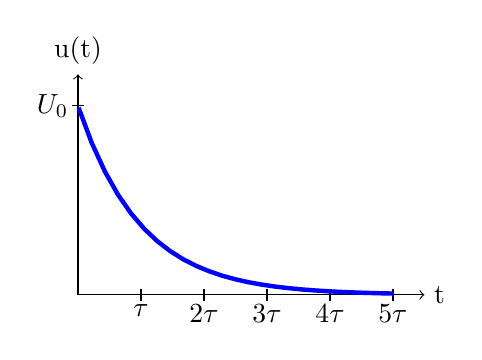
\begin{tikzpicture}[xscale=0.8, yscale=0.8]
	%\draw[help lines] (0,0) grid (6,4);
	\normalsize
	\draw [<->] (0, 3.5) -- (0, 0) -- (5.5, 0);
	\node [right] at (5.5, 0) {t};
	\node [above] at (0, 3.5) {u(t)};
	
	\draw (1, -0.1) --  (1, 0.1);
	\node [below] at (1, 0) {$\tau$};
	\draw (2, -0.1) --  (2, 0.1);
	\node [below] at (2, 0) {$2\tau$};
	\draw (3, -0.1) --  (3, 0.1);
	\node [below] at (3, 0) {$3\tau$};
	\draw (4, -0.1) --  (4, 0.1);
	\node [below] at (4, 0) {$4\tau$};
	\draw (5, -0.1) --  (5, 0.1);
	\node [below] at (5, 0) {$5\tau$};
	
	
	\node [left] at (0, 3) {$U_0$};
	\draw (-0.1, 3) --  (0.1, 3);
	\draw[blue, ultra thick, domain=0.01:5] plot (\x, {3*e^(-\x)});
\end{tikzpicture}
}
  	\begin{center}
  		\huge
  		$u(t) = U_0 \cdot e^{-\frac{t}{\tau}} $
  	\end{center}
\end{karte}

\begin{karte}{Wie heisst die Gleichung der folgender Entladefunktion?\\ %Autor: Simon Walker
%Version: 1.0
%Datum: 10.11.2019

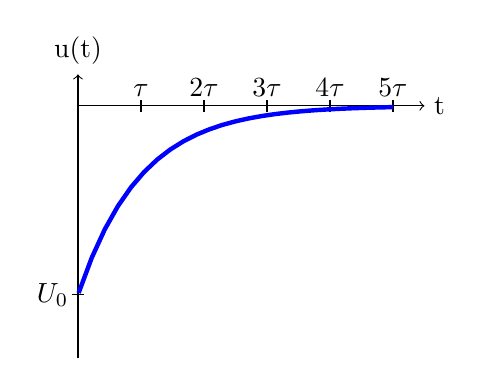
\begin{tikzpicture}[xscale=0.8, yscale=0.8]
	%\draw[help lines] (0,0) grid (6,4);
	\normalsize
	\draw [->] (0, 4) -- (0, 4.5);
	\draw [<-] (5.5, 4) --  (0, 4) -- (0, 0);
	\node [right] at (5.5, 4) {t};
	\node [above] at (0, 4.5) {u(t)};
	
	\draw (1, 3.9) --  (1, 4.1);
	\node [above] at (1, 4) {$\tau$};
	\draw (2, 3.9) --  (2, 4.1);
	\node [above] at (2, 4) {$2\tau$};
	\draw (3, 3.9) --  (3, 4.1);
	\node [above] at (3, 4) {$3\tau$};
	\draw (4, 3.9) --  (4, 4.1);
	\node [above] at (4, 4) {$4\tau$};
	\draw (5, 3.9) --  (5, 4.1);
	\node [above] at (5, 4) {$5\tau$};
	
	
	\node [left] at (0, 1) {$U_0$};
	\draw (-0.1, 1) --  (0.1, 1);
	\draw[blue, ultra thick, domain=0.01:5] plot (\x, {(-3)*e^(-\x) + 4});
\end{tikzpicture}
}
	\begin{center}
		\huge
		$u(t) = U_0 \cdot e^{-\frac{t}{\tau}} $\\[10pt]
		\normalsize
		Wobei $U_0$ negativ ist.
	\end{center}
\end{karte}

\begin{karte}{Wie heisst die Gleichung der folgender Ladefunktion?\\ %Autor: Simon Walker
%Version: 1.0
%Datum: 10.11.2019

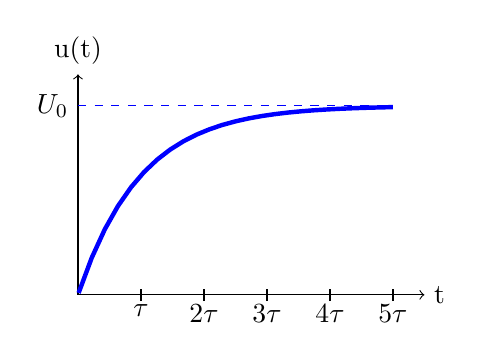
\begin{tikzpicture}[xscale=0.8, yscale=0.8]
	%\draw[help lines] (0,0) grid (6,4);
	\normalsize
	
	\draw [<->] (0, 3.5) -- (0, 0) -- (5.5, 0);
	\node [right] at (5.5, 0) {t};
	\node [above] at (0, 3.5) {u(t)};
	
	\draw (1, -0.1) --  (1, 0.1);
	\node [below] at (1, 0) {$\tau$};
	\draw (2, -0.1) --  (2, 0.1);
	\node [below] at (2, 0) {$2\tau$};
	\draw (3, -0.1) --  (3, 0.1);
	\node [below] at (3, 0) {$3\tau$};
	\draw (4, -0.1) --  (4, 0.1);
	\node [below] at (4, 0) {$4\tau$};
	\draw (5, -0.1) --  (5, 0.1);
	\node [below] at (5, 0) {$5\tau$};
	
	\draw [dashed, blue] (0, 3) -- (5, 3);
	\node [left] at (0,3) {$U_0$};
	\draw[blue, ultra thick, domain=0.01:5] plot (\x, {3*(1-e^(-\x))});
	
\end{tikzpicture}
}
	\begin{center}
		\huge
		$u(t) = U_0 \cdot (1 - e^{-\frac{t}{\tau}}) $
	\end{center}
\end{karte}

\begin{karte}{Wie lautet die Differenzialgleichung des Kondensators und was folgt daraus?}
	\begin{center}
		\huge
		$\frac{d u_{C}}{d t}=\frac{i_{C}}{C}$
	\end{center}
	\begin{itemize}
		\item Strom durch einen Kondensator bedingt einer Spannungsänderung
		\item Bei einem grossen Kondensator $(C \gg 0)$ führen auch grosse Ströme nur zu relativ kleinen Spannungsänderungen.
		\item Eine grosse Spannungsänderung an einem Kondensator bedingt einem grossen Strom oder einer kleinen Kapazität
	\end{itemize}
	
\end{karte}

\begin{karte}{Wie kann die Spannung $u_C(t)$ berechnet werden wenn zum Zeitpunkt $t_0$ der Schalter geschlossen wird?\\[10pt] %Autor: Simon Walker
%Version: 1.0
%Datum: 10.11.2019

\begin{tikzpicture}[scale=0.7, every node/.style={scale=0.7}]
%\draw[help lines] (0,0) grid (9, 5);
\normalsize

% Spannungsquelle
\tzUV{0.5}{2.5}{$U_0$}{r}{+}

% Leitungen
%U0 - SW
\draw (0.5, 3) -- (0.5, 4.5) -- (1.4, 4.5);
%SW - R1
\draw (2.6, 4.5) -- (4.5-0.7, 4.5);
%R1 - C
\draw (5.2, 4.5) -- (7.5, 4.5) -- (7.5, 2.75);
\tzKN{6}{4.5} %Knoten 1
%Knoten1 - R_2
\draw (6, 4.5) -- (6, 3.2);
%R2 - Knoten2
\draw (6, 1.8) -- (6, 0.5);
\tzKN{6}{0.5} %Knoten 2
%C - U0
\draw (0.5, 2) -- (0.5, 0.5) -- (7.5, 0.5) -- (7.5, 2.25);

%Schalter (Schliesser)
\tzSH{2}{4.5}

% Widerstand R1
\tzRH{4.5}{4.5}{$R_1$}{b}

% Widerstand R2 (mitte 5.5, 2.5)
\tzRV{6}{2.5}{$R_2$}{l}

% Kondensator C (mitte 7.5, 2.5)
\tzCV{7.5}{2.5}{$C$}{l}	

% Spannungspfeil über Kondensator
\draw [->,thick ,blue] (8.5, 3.5) to [out=-70, in=70] (8.5, 1.5); 
\node [blue, right] at (8.7, 2.5) {\Large $u_C(t)$};


\end{tikzpicture}}
	1. Ersatzspannungsquelle berechnen für den geschlossenen Schalter.\\
	\begin{minipage}{0.6\textwidth}
		%Autor: Simon Walker
%Version: 1.0
%Datum: 10.11.2019

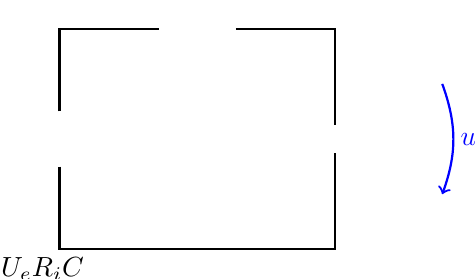
\begin{tikzpicture}[thick,scale=0.7, every node/.style={scale=0.7}]%[xscale=0.6, yscale=0.6]
	
	%\draw[help lines] (0,0) grid (9, 5);
	\normalsize
	
	% Spannungsquelle
	\tzUV{0.5}{2.5}{$U_e$}{r}{+}
	
	% Leitungen
	%Ue - Ri
	\draw (0.5, 3) -- (0.5, 4.5) -- (2.3, 4.5);
	%Ri - C
	\draw (3.7, 4.5) -- (5.5, 4.5) -- (5.5, 2.75);
	%C - Ue
	\draw (0.5, 2) -- (0.5, 0.5) -- (5.5, 0.5) -- (5.5, 2.25); 
	
	% Widerstand R1
	\tzRH{3}{4.5}{$R_i$}{b}
		
	% Kondensator C (mitte 7.5, 2.5)
	\tzCV{5.5}{2.5}{$C$}{l}
	
	% Spannungspfeil über Kondensator
	\draw [->,thick ,blue] (6.5, 3.5) to [out=-70, in=70] (6.5, 1.5); 
	\node [blue, right] at (6.7, 2.5) {\Large $u_C(t)$};
	
	
\end{tikzpicture}

	\end{minipage}
	\begin{minipage}{0.4\textwidth}
		$R_i = \dfrac{R_1\cdot R_2}{R_1+R_2}$\\[5pt]
		$U_e = U_0 \cdot \dfrac{R_2}{R_1 + R_2}$
	\end{minipage}
	2. Spannung $u_C$ berechnen.\\
	$ u_C(t)= U_e \cdot \left(1-e^{\frac{-t}{\tau}}\right)$

\end{karte}

\begin{karte}{Was ist ein Verschiebungsstrom?}
	\begin{center}
		\begin{itemize}
			\item 	Kirchhof ist nicht mehr allgemein gültig. Denn es kann sich nun auch Ladung ansammeln.\\
			\begin{equation*}
			\displaystyle \oint_{\text {Hülle }} \vec{J} \cdot d \vec{s}=0 \quad \Leftrightarrow \quad  \sum_{n} I_{n}=0
			\end{equation*}
			Deshalb muss nun Kirchhof mit dem Verschiebungsstrom erweitert werden:\\
			\begin{equation*}
			\displaystyle \oint_{\text {Hülle }} \vec{J} \cdot d \vec{s}+\frac{d Q_{\text {eingeschlossen }}}{d t}(t)=0
			\end{equation*}
			\item Der Verschiebungsstrom verursacht ebenfalls ein Magnetfeld!
		\end{itemize}
	\end{center}
\end{karte}	


